\section{Обучение нейросети по некомплектным данным}

Отсутствие значений в данных (\emph{пропуски}) представляет собой одну из наиболее распространённых и при этом наименее формализованных проблем, с которой сталкиваются в прикладном машинном обучении и статистическом анализе. Согласно \cite{little1995statistical}, в любой области, где данные собираются при помощи опросов, сенсоров или в рамках наблюдательных исследований, практически неизбежно возникает неполнота -- отсутствие значений некоторых признаков у части объектов выборки. Такая ситуация наблюдается в биомедицинских данных~\cite{cismondi2013missing}, социологических опросах, прикладных инженерных задачах, финансовом моделировании и других областях.

Пропуски могут быть обусловлены множеством факторов: техническими сбоями~\cite{du2020missing}, отказами респондентов отвечать на конкретные вопросы, ограничениями ресурсоёмких измерений, фильтрацией данных, нарушениями сбора и хранения. При этом даже небольшое число пропущенных значений может существенно повлиять на результаты анализа, особенно при высокой размерности признакового пространства или в задачах, чувствительных к структуре выборки.

Корректное обращение с пропущенными значениями требует не только выбора соответствующей стратегии заполнения, но и понимания механизма возникновения пропусков. Как подчёркивается в \cite{little1995statistical, schafer1997analysis}, пренебрежение механизмом отсутствия может привести к систематическим ошибкам, смещению оценок, снижению статистической мощности и искажению выводов. Особенно это критично в задачах обучения нейросетей, где входные данные передаются в модели в виде числовых векторов, не допускающих наличия неопределённых компонент.

\subsection{Задача классификации данных с пропущенными значениями}

Пусть имеется обучающая выборка из \(n\) объектов: \( \{(X_i, Y_i)\}_{i=1}^n \), где \(X_i \in [0, 1]^d\) -- вектор признаков, а \(Y_i \in \{1, 2, \dots, C\}\) -- метка класса. Предполагается, что некоторые признаки могут быть пропущены. Для описания структуры отсутствующих данных вводится матрица \(M \in \{0, 1\}^{n \times d}\), где \(m_{ij} = 1\) означает, что признак \(j\) отсутствует у объекта \(i\), а \(m_{ij} = 0\) -- признак наблюдаем.

Обозначим через \(X_0\) множество наблюдаемых признаков, а через \(X_1\) -- множество отсутствующих.

\subsection{Типы механизмов пропусков}

Следуя формализации, приведённой в \cite{little1995statistical}, различают три основных типа пропусков:

\begin{itemize}
    \item Пропуски, отсутствующие полностью случайно (MCAR, missing completely at random): механизм пропусков не зависит ни от наблюдаемых, ни от ненаблюдаемых данных. Формально, \(P(M \mid X_0, X_1, Y) = P(M)\).
    \item Пропуски, отсутствующие случайно (MAR, missing at random): вероятность отсутствия значения может зависеть от наблюдаемых данных, но не от пропущенных. То есть \(P(M \mid X_0, X_1, Y) = P(M \mid X_0, Y)\).
    \item Пропуски, отсутствующие не случайно (NMAR, not missing at random): вероятность отсутствия значения зависит от ненаблюдаемых данных, т.е. \(P(M \mid X_0, X_1, Y)\) не сводится к предыдущим случаям.
\end{itemize}

При предположении MCAR и MAR допускается игнорирование механизма пропусков при построении модели. В случае NMAR необходимо явно моделировать процесс отсутствия данных, что усложняет задачу.

\subsection{Существующие методы обработки пропусков}

В литературе представлены различные стратегии, позволяющие бороться с неполнотой данных. Кратко охарактеризуем наиболее известные из них.

\subsubsection{Удаление некомплектных наблюдений}

Простейший метод -- исключение строк с пропущенными значениями. Такой подход корректен только при MCAR и при условии, что доля удаляемых объектов незначительна. Основной недостаток -- потеря потенциально полезной информации и возможное смещение выборки.

\subsubsection{Заполнение средним значением (mean imputation)}

Отсутствующие значения заменяются средним по соответствующему признаку, вычисленным по доступным наблюдениям:
\[
x_{ij} \leftarrow \frac{1}{|\mathcal{I}_j|} \sum_{i \in \mathcal{I}_j} x_{ij}, \quad \mathcal{I}_j = \{ i \mid m_{ij} = 0 \}.
\]
Метод не учитывает зависимость между признаками, занижает дисперсию и нарушает ковариационную структуру данных.

\subsubsection{Заполнение медианой или модой}

Применяется для категориальных признаков (мода) или числовых с выбросами (медиана). Устраняет чувствительность к экстремальным значениям, но по-прежнему игнорирует корреляции и структуру признаков.

\subsubsection{\(k\)-ближайших соседей (kNN imputation)}

Для объекта с пропущенным признаком ищется множество \(k\) ближайших (по наблюдаемым координатам) объектов, и пропущенное значение заполняется агрегатом (среднее, медиана) по этому множеству. Обозначим через \( \mathcal{N}_k(i) \) множество \(k\)-соседей объекта \(i\). Тогда:
\[
x_{ij} \leftarrow \frac{1}{k} \sum_{\ell \in \mathcal{N}_k(i)} x_{\ell j}.
\]
Метод чувствителен к выбору метрики, неустойчив при высокой разреженности и требует полного набора значений для вычисления расстояний~\cite{pujianto2019k}.

\subsubsection{Множественное заполнение и EM-алгоритм}

В рамках подхода максимального правдоподобия в \cite{dempster1977maximum} вводится вероятностная модель данных и итеративно оцениваются параметры и пропущенные значения. На шаге \textbf{E} оценивается распределение некомплектных данных при фиксированных параметрах, на шаге \textbf{M} -- параметры по комплектным данным. Подход требует априорных предположений о распределении данных (обычно гауссовское) и высоких вычислительных затрат. В случае множественного заполнения \cite{rubin1988overview} создаётся несколько возможных вариантов с последующей агрегацией.

\subsubsection{Методы на основе PCA и автокодировщиков}

Пропуски заполняются с помощью аппроксимации данных в латентном пространстве. В методах PCA недостающие значения восстанавливаются проекцией на подпространство главных компонент~\cite{moh2024missing}. В нейросетевом варианте -- автокодировщики обучаются на комплектных данных и используются для реконструкции пропущенных~\cite{roskams2023leveraging}.

\subsection{Ограничения классических методов}

Все перечисленные методы обладают рядом общих недостатков:
\begin{itemize}
    \item не учитывают апостериорную неопределённость заполнения;
    \item вводят систематическое смещение в оценки параметров модели;
    \item теряют вариативность по заполненным признакам;
    \item игнорируют структуру задачи (например, наличие классов в классификации).
\end{itemize}

Таким образом, возникает необходимость в методах, которые позволяли бы обрабатывать некомлпектные данные без грубых аппроксимаций, использовали бы информацию о метках классов и сохраняли бы стохастический характер восстановления недостающих признаков.

В работе~\cite{perminov2025missing} предлагается альтернативный метод, основанный на вероятностном заполнении признаков с помощью унарной классификации и многослойного персептрона.

\subsection{Метод вероятностного заполнения}

Пусть \(X \in [0, 1]^{n \times d}\) -- обучающая выборка с пропущенными значениями, \(Y \in \{0, 1, \dots, C\}^n\) -- вектор меток классов, \(M \in \{0, 1\}^{n \times d}\) -- матрица пропусков. Предполагается, что механизм пропусков является случайным (MCAR или MAR по классификации Рубина~\cite{little1995statistical}).

Предлагаемый метод обучения MLP при наличии пропусков в обучающей выборке применяется последовательно к каждому из \(C\) классов и состоит из трёх шагов (схематичное изображение методики изображено на рисунке~\cref{fig:missing_diagram}):

\begin{enumerate}

    \item \textbf{Начальное обучение.} Для комплектной подвыборки \(\{X\}_i^n\) \(j\)-го класса, \(j \in \{1, 2, \cdots C\}\), решить задачу унарной классификации и построить персептрон, реализующий кусочно-линейную непрерывную функцию \(c_n^{(j)}(X)\).
    
    \item \textbf{Дообучение.} Дообучение  осуществляется по всей обучающей выборке \(j\)-го класса отдельными эпохами. Перед текущей эпохой выполнить временное (для данной эпохи) заполнение некомплектных наблюдений. Для каждого некомплектного наблюдения \(X\):

    \begin{enumerate}
        \item Разделить множество индексов координат вектора \(X=(x_1, x_2, \cdots, x_d)\) на два подмножества \(M_0\) и \(M_1\), включающие соответственно индексы заполненных и пропущенных координат. 
        
        \item Заполнить координаты \(X\) из \(M_1\) наблюдениями равномерно распределенной случайной величины на отрезке \([0, 1]\), в результате чего будет получен комплектный вектор \(X'\). Вычислить \(c_n^{(j)}(X')\). Сгенерировать наблюдение биномиальной случайной величины с вероятностью успеха \(p=c_n^{(j)}(X')\).
        
        \item При успешном исходе временно заменить в обучающей выборке некомплектный вектор \(X\) на комплектный вектор \(X'\) и перейти к рассмотрению следующего некомплектного наблюдения. В противном случае повторить предыдущий шаг.
        
        \item Выполнить дообучение сети по ``доукомплектованной`` обучающей выборке.
    \end{enumerate}
    
    \item Перейти к следующей эпохе дообучения, повторяя шаги а-г, до полного завершения обучения \(MLP_j\) для \(j\)-го класса с функцией нейросетевой регрессии \(c_n^{(j)}(X)\).
\end{enumerate}

Повторяя шаги 1-3 для всех классов, получим \(C\) обученных нейросетей \(MLP_j\) и соответствующих им непрерывных кусочно-линейных функций \(\{c_n^{(1)}(X), c_n^{(2)}(X), \cdots, c_n^{(C)}(X)\}\), каждая из которых есть выборочная оценка апостериорной вероятности соответствующего класса в точке \(X\).

\begin{figure}[ht]
    \centerfloat{
        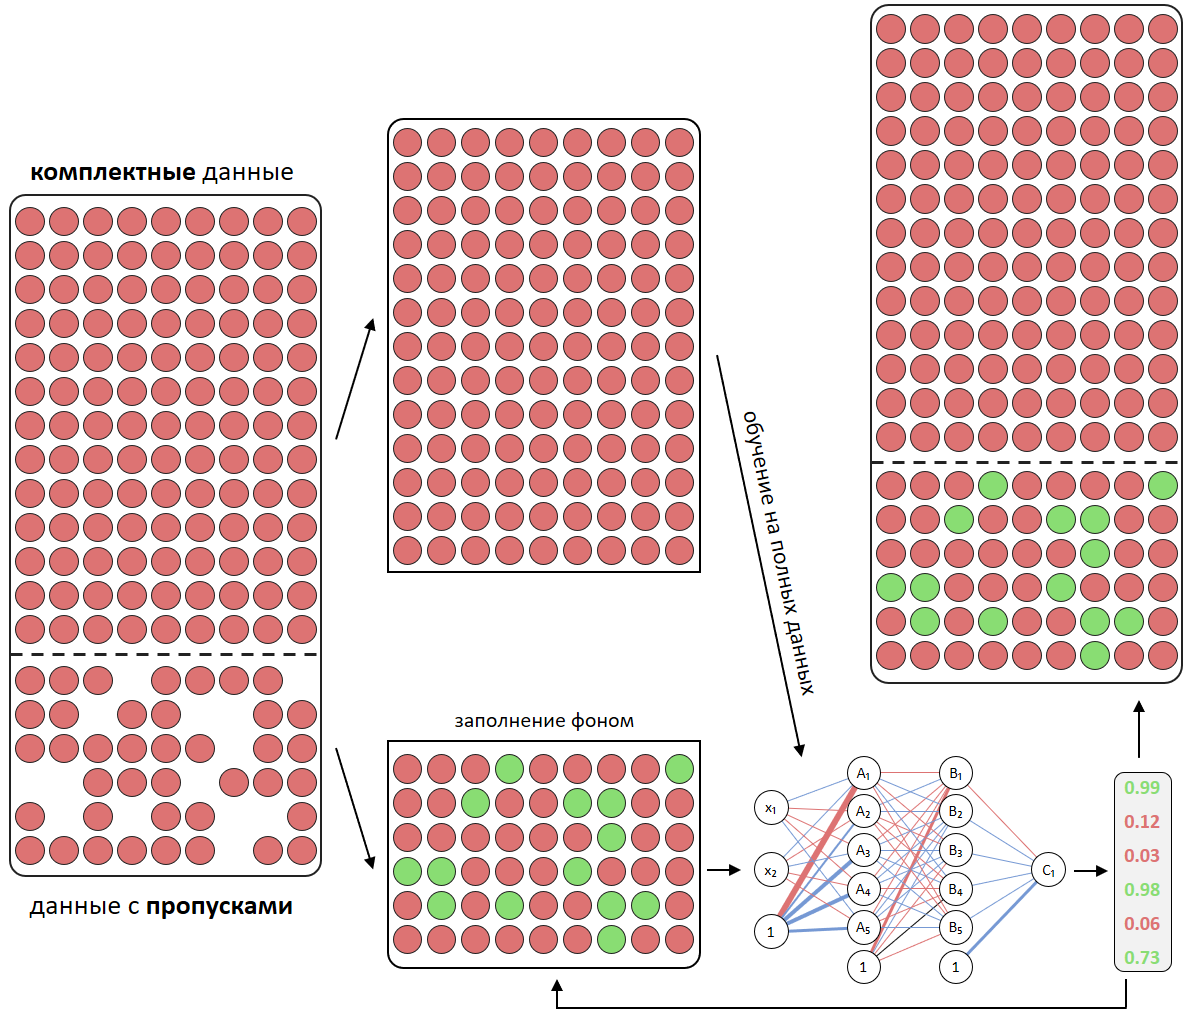
\includegraphics[width=\linewidth]{Dissertation/images/ch3/missing_data/diagram.png}
    }
    \caption{Схема обучения \(c_n^{(j)}(X)\) по некомплектным данным}
    \label{fig:missing_diagram}
\end{figure}


\subsection{Классификация комплектного наблюдения}

Для решения задачи классификации комплектного наблюдения \(X\) возможны различные стратегии. Простейшая состоит в выборе класса, для которого апостериорная вероятность максимальна. Другой вариант -- выбрать в качестве решения все классы, значения апостериорной вероятности для которых больше некоторого заданного порога, и продолжить решение задачи классификации, например, в другом признаковом пространстве.

\subsection{Экспериментальное исследование}

Для экспериментального анализа были подготовлены несколько модельных наборов данных с чёткой визуальной и статистической интерпретацией классов. Это позволило обеспечить контролируемую среду и надёжную оценку устойчивости моделей к пропущенным значениям.

\subsubsection{Используемые наборы данных}
\begin{itemize}
    \item \textbf{Гауссианы} -- два нормально распределённых кластера с равной дисперсией и небольшим перекрытием (рисунок~\cref{fig:missed_datasets}\subcaptionref{fig:missed_datasets_gaussians}).
    \item \textbf{Спирали} -- классы формируют витки спиралей с общей точкой начала координат, разделение классов сильно нелинейное (рисунок~\cref{fig:missed_datasets}\subcaptionref{fig:missed_datasets_spiral}).
    \item \textbf{Кольцо и круг} -- один класс расположен внутри круга, второй образует кольцо с зазором между границами (рисунок~\cref{fig:missed_datasets}\subcaptionref{fig:missed_datasets_circle}).
\end{itemize}

\begin{figure}[ht]
    \centerfloat{
        \hfill
        \subcaptionbox{Гауссианы\label{fig:missed_datasets_gaussians}}{%
            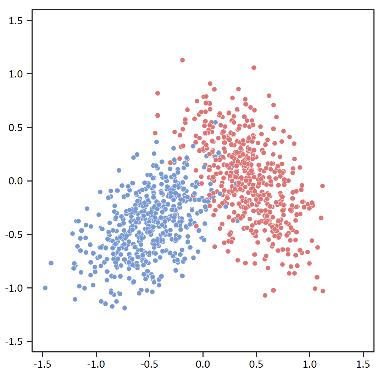
\includegraphics[width=0.32\linewidth]{Dissertation/images/ch3/missing_data/gaussians.png}}
        \hfill
        \subcaptionbox{Спираль\label{fig:missed_datasets_spiral}}{%
            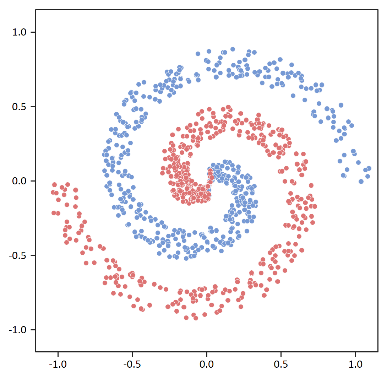
\includegraphics[width=0.32\linewidth]{Dissertation/images/ch3/missing_data/spirals.png}}
        \hfill
        \subcaptionbox{Кольцо и круг\label{fig:missed_datasets_circle}}{%
            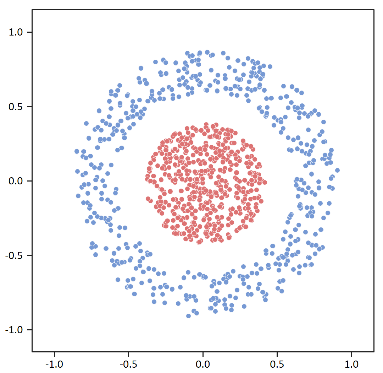
\includegraphics[width=0.32\linewidth]{Dissertation/images/ch3/missing_data/circles.png}}
        \hfill
    }
    \caption{Использованные наборы для обучения модели на данных с пропусками}
    \label{fig:missed_datasets}
\end{figure}

\subsubsection{Обработка пропущенных значений}
Во всех наборах данных искусственно вводились пропуски в признаках с уровнями 20\%, 40\%, 50\%, 60\%, 80\% и 90\%. Пропуски вносились случайно и только в признаках (целевые метки всегда сохранялись). Были рассмотрены следующие классические методы обработки пропусков:

\begin{itemize}
    \item \textbf{mean} -- заполнение по среднему значению признака;
    \item \textbf{mode} -- заполнение наиболее частым значением;
    \item \textbf{\(kNN (k=3)\)} -- заполнение по ближайшим трём соседям в евклидовом пространстве;
    \item \textbf{\(kNN (k=7)\)} -- аналогично, но с \(k=7\);
    \item \textbf{reproduction} (предложенный метод) -- метод, основанный на унарной классификации.
\end{itemize}

\subsubsection{Сценарии обучения}
Для каждой комбинации набора данных и уровня пропусков модель обучалась в следующих режимах:

\begin{itemize}
    \item \textbf{full} -- обучение на полном наборе без пропусков;
    \item \textbf{complete} -- обучение только на тех примерах, где отсутствуют пропуски;
    \item \textbf{imputed} -- обучение на наборе, где пропуски заполнялись одним из методов.
\end{itemize}

В качестве модели использовался многослойный персептрон с \(L=2\) скрытыми слоями по \(k=20\) нейронов в каждом и одним выходным слоем. Обучение осуществлялось на протяжении 500 эпох.

Каждая комбинация набора данных, уровня пропусков и метода заполнения запускалась 50 раз с различными начальными инициализациями весовых коэффициентов. В качестве основной метрики использовалась точность классификации (accuracy) на тестовом множестве из соответствующего набора данных из 5000 элементов. Все тестовые наборы содержали только комплектные данные.

Для метода репродукции персептрон обучался в течение 50 эпох на данных без пропусков, а затем каждую эпоху запускался процесс вероятностного заполнения пропусков и обучение продолжалось уже на обновлённых заполненных данных.

\subsubsection{Результаты}
Сводные таблицы \cref{tab:missing_results_gaussians}, \cref{tab:missing_results_spiral} и \cref{tab:missing_results_circle} по accuracy (в среднем по 50 запускам) представлены ниже. Визуальный анализ показывает, что метод репродукции демонстрирует более высокую устойчивость при высоких уровнях пропусков, особенно на сложных наборах данных, как например "кольцо и круг". Традиционные методы заполнения (среднее, мода) показывают ожидаемое снижение качества, особенно при пропусках выше 60\%. Метод \(kNN\) даёт умеренное улучшение, но чувствителен к плотности выборки.

\begin{table} [htbp]
    \centering
    \begin{threeparttable}
        \caption{Оценка метода репродукции для заполнения пропусков на наборе данных ``Гауссианы``}\label{tab:missing_results_gaussians}
        \begin{SingleSpace}
        \begin{tabular}{|c|c|c|c|c|c|}
            \hline
            Доля & full & complete & reproduce & mean & knn 7 \\
            \hline
            20\% &       & 0.919±0.006 & \textbf{0.925±0.004} & 0.917±0.007 & 0.921±0.006 \\
            40\% &       & \textbf{0.919±0.006} & 0.917±0.009 & 0.897±0.008 & 0.915±0.005 \\
            50\% & 0.925 & 0.917±0.005 & \textbf{0.918±0.008} & 0.904±0.014 & 0.917±0.005 \\
            60\% &   ±   & 0.910±0.013 & \textbf{0.921±0.009} & 0.866±0.018 & 0.894±0.012 \\
            80\% & 0.003 & 0.875±0.011 & \textbf{0.912±0.008} & 0.752±0.047 & 0.851±0.011 \\
            90\% &       & 0.842±0.023 & \textbf{0.906±0.007} & 0.593±0.092 & 0.806±0.015 \\
            \hline
        \end{tabular}
        \end{SingleSpace}
    \end{threeparttable}
\end{table}


\begin{table} [htbp]
    \centering
    \begin{threeparttable}
        \caption{Оценка метода репродукции для заполнения пропусков на наборе данных ``Спираль``}\label{tab:missing_results_spiral}
        \begin{SingleSpace}
        \begin{tabular}{|c|c|c|c|c|c|}
            \hline
            Доля & full & complete & reproduce & mean & knn 7 \\
            \hline
            20\% &       & 0.936±0.031 & \textbf{0.945±0.025} & 0.922±0.032 & 0.941±0.020 \\
            40\% &       & 0.924±0.023 & \textbf{0.930±0.021} & 0.899±0.034 & 0.918±0.025 \\
            50\% & 0.941 & \textbf{0.926±0.016} & 0.910±0.034 & 0.893±0.031 & 0.868±0.062 \\
            60\% &   ±   & \textbf{0.913±0.030} & 0.898±0.047 & 0.890±0.027 & 0.853±0.040 \\
            80\% & 0.024 & \textbf{0.869±0.039} & 0.861±0.044 & 0.750±0.095 & 0.773±0.062 \\
            90\% &       & \textbf{0.827±0.042} & 0.812±0.067 & 0.545±0.082 & 0.695±0.040 \\
            \hline
        \end{tabular}
        \end{SingleSpace}
    \end{threeparttable}
\end{table}

\begin{table} [htbp]
    \centering
    \begin{threeparttable}
        \caption{Оценка метода репродукции для заполнения пропусков на наборе данных ``Кольцо и круг``}\label{tab:missing_results_circle}
        \begin{SingleSpace}
        \begin{tabular}{|c|c|c|c|c|c|}
            \hline
            Доля & full & complete & reproduce & mean & knn 7 \\
            \hline
            20\% &       & 0.987±0.009 & \textbf{0.989±0.006} & 0.941±0.058 & 0.927±0.086 \\
            40\% &       & 0.984±0.011 & \textbf{0.986±0.011} & 0.865±0.103 & 0.846±0.123 \\
            50\% & 0.981 & 0.971±0.019 & \textbf{0.984±0.016} & 0.852±0.094 & 0.751±0.149 \\
            60\% &   ±   & 0.974±0.018 & \textbf{0.981±0.016} & 0.763±0.083 & 0.705±0.103 \\
            80\% & 0.014 & 0.892±0.136 & \textbf{0.964±0.031} & 0.609±0.148 & 0.618±0.069 \\
            90\% &       & 0.852±0.080 & \textbf{0.952±0.038} & 0.295±0.126 & 0.562±0.055 \\
            \hline
        \end{tabular}
        \end{SingleSpace}
    \end{threeparttable}
\end{table}